\documentclass[12pt]{article}

\setlength{\parindent}{0pt}
\setlength{\parskip}{2mm}

\usepackage{geometry}
 \geometry{
 letterpaper, left=20mm, right=20mm,  top=20mm,
 }
\usepackage{graphicx}
\graphicspath{ {graphics/} }
\usepackage{amssymb}

%%%%%%%%%%%%%%%%%%%%%%%%%%%%%%%%%%%%%%%%%%%%%%%%%
\title{RFC 1: Collisions in Delay-Based ID Encoding Protocol}
%%%%%%%%%%%%%%%%%%%%%%%%%%%%%%%%%%%%%%%%%%%%%%%%%

\author{
	Margot Maxwell \and
	Lizzy Schoen \and
	Noah Strong \and
	Chloe Yugawa
}

\date{v1.2 -- \today}

\begin{document}

\maketitle

\tableofcontents{}

%%%%%%%%%%%%%%%%%%%%%%%%%%%%%%%%%%%%%%%%%%%%%%%%%

\section{Introduction}

The protocol proposed for this project encodes a unique identification number
in the transmitted signal by the delay between two consecutive pings.
While this method is easy to implement in hardware, and works well in the case
of only a signal transmitter, the addition of multiple transmitters within range
of a receiver brings about the potential for collisions between different
signals.
In some cases, the collisions may be undetectable, leading to incorrect
reporting of nearby crab IDs.
Completely solving this problem will require a change to the underlying
protocol.
However, the likelihood of such collisions may be low enough that we can move
forward with this known flaw in the protocol.

\section{Original Protocol}

In the current iteration of our detection and identification protocol, every
transmitter will transmit at the exact same frequency, somewhere around
40kHz. This is ideal from a hardware perspective, as the piezoelectric
equipment can be tuned to work on a single frequency with a high degree of
accuracy.

Every transmitter will periodically send out two quick ``pings,'' each separated
by some delay $d$. The value of $d$ will encode the ID of the transmitter.
For example, $d=42$ms may correspond to ID 30, while $d=50.5$ms may
correspond to an ID of 38.
Note that these numbers are only for illustration purposes.
Because the receiving hardware can easily detect the two pings, it can measure
the value of $d$ by calculating the time difference between the rising edges
of the consecutive signals. See Figure 1 for an illustration.

\begin{figure}[h]
\centering
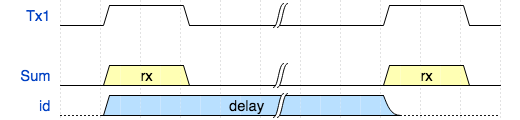
\includegraphics[scale=0.7]{singleTx}

\caption{A single transmitter ($Tx1$), the input received by the receiver
($Sum$), and the calculated delay $d$ based on the time measured between
the rising edges of the two pings from $Tx1$.}
\end{figure}

Each transmission of an ID by a transmitter (that is, the sequence of a
ping, a delay, and another ping) will happen regularly around some average
interval.
Because there is no synchronization between transmitters, the interval
between each broadcast will vary randomly within a given range.
For example, the delay may be 30 seconds, $\pm$5 seconds, with the random
variation recalculated after every broadcast.

The motivation behind the randomly-varying schedule is to decrease the
likelihood of simultaneous transmissions by two different receivers.
However, the random interval only functions to reduce the likelihood of
two \emph{consecutive} overlapping transmissions.
Without an inter-receiver collision-detection solution, there will always
be the possibility that two transmissions overlap.

\section{Possibility for Collisions}

As discussed above,
when two transmitters are present in the receiving range, and there is no
synchronization between the two (i.e. they may transmit their IDs at any
time, regardless of when the other transmits), it is possible for the two
transmissions to be broadcast at similar times, thereby overlapping.
The signals may overlap in countless different ways depending on when
both transmissions start and where the transmitters are in relation to
each other and to the receiver.

In some cases, collisions may cause the data to be some so skewed that it will
be easy to detect and throw away. However, in a more likely and more dangerous
situation, the overlap of data will lead to inaccurate results and be extremely
difficult to detect.

\subsection{Example Scenarios}

Below are a few possible scenarios that may occur in practice or in testing
environments. Note that this is by no means an exhaustive list, but instead
a selection of cases chosen to demonstrate potential issues.

We'll define some notation for the sake of convenience and clarity.
If $Tx1$ is a transmitter, then $d_1$ is the delay time between
the two pings for $Tx1$; that is, $d_1$ encodes the unique ID for $Tx1$.
We'll also use $B_1$ to denote the first ping from $Tx1$
(the {\bf B}eginning of the encoding) and $E_1$ to denote the second
({\bf E}nd of the encoding) ping.

\subsubsection{Close Proximity, Similar Start}

{\bf Situation:} Two transmitters in close proximity to each other transmit at
very nearly the same time.
Their transmissions line up so that the first ping from $Tx2$ starts as the
first ping from $Tx1$ is broadcasting.
If the delay times happen to be very similar for the two transmitters,
it is possible that the same effect is observed in reverse on the ending
pings. That is, the second ping for $Tx2$ begins just before the second ping
for $Tx1$. See Figure 2 for an illustration.

{\bf Potential Effect:}
Should this happen, the receiver will register two pings, just as it would if
only one transmitter broadcasts. However, the measured delay
$d_{measured}$ will not equal $d_1$ or $d_2$.
Thus the software will report the ID corresponding to $d_{measured}$, and
not the ID of either of the transmitters actually broadcasting. Worse still,
there is no way to detect when this happens.

\begin{figure}[h]
	\centering
		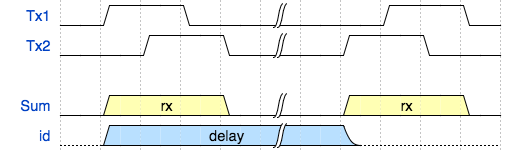
\includegraphics[scale=0.7]{collision1}
		
		\caption{An example collision. The computed delay $d$ is
		measured as the time difference between the rising edge of
		$Tx1$'s first ping and $Tx2$'s second ping.}
\end{figure}

\subsubsection{Close Proximity, Offset Broadcasts}

{\bf Situation:} As in the previous example, suppose there are two transmitters
in close proximity to each other.
However, in this situation, suppose the two transmissions are broadcast at
similar times so that they are interleaved.
That is, the receiver will see $B_1$, $B_2$, $E_1$, $E_2$, in that order.
See Figure 2 for an illustration.

{\bf Potential Effect:}
In this case, the receiver will detect two different delay times, which may
seem normal. However, these delays are once again wrong -- they do not
correspond to any transmitter actually transmitting.
The software will then report that there are two signals coming from a
specific direction, but the IDs that it thinks these correspond to will
be incorrect.
As in the previous example, there is no way to detect when this happens, so the
software would unknowingly present incorrect information.

\begin{figure}[h]
	\centering
		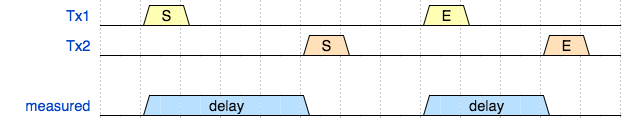
\includegraphics[scale=0.7]{collision2}
		
		\caption{Another example collision. Note that in this situation,
		two distinct delays are measured. While it is possible for them
		to both correlate to valid IDs, neither delay matches the delays
		actually encoded by $Tx1$ or $Tx2$.}
\end{figure}

\subsubsection{A Series of Overlapping Broadcasts}

In an extreme case, it may be possible for multiple transmitters to all begin
broadcasting at very similar times such that all of their pings overlap and are
registered as a single (extremely long) ping.
For instance, if $n$ transmitters send out pings perfectly sequentially,
it is conceivable
that the receiver receives $B_1$, $B_2$, $\dots$, $B_n$ in order with so little
temporal separation that no falling edges are registered by the receiving
hardware.
In other words, the receiver hears one long, solid tone, as opposed to a series
of quick pings. It is theoretically possible that this single perceived tone
is so long that the ending pings of one or more transmitters may be hidden.

This is an extreme case, but is nonetheless a possibility given significant
transmitter density in the receiving range, sufficiently long pings, and
sufficiently low delay $d_n$ values for the transmitters in play.

\subsubsection{Mutually Distant Transmitters}

In general, though the above situations are quite possible, it is more likely
that two or more transmitters in the receiving range will be in different
directions from the receiving station.
When two or more transmitters that are in different areas around the receiver
broadcast at similar times, the overlaps will interfere in even more complex
ways.
Such scenarios are much more difficult to illustrate, but suffice it to say
that they will also cause problems with invalid or confusing data.
As before, some collisions can be detected and compensated for with a
sufficiently complex algorithm, but not all cases are solvable with the current
protocol.

\section{Potential Solutions}

Some early solutions that do not entirely change the original protocol have
been proposed. They are discussed briefly below. This section may be expanded
in the future as we discuss more options.

\subsection{Use Two Frequencies To Differentiate Pings}

One proposed solution is for every transmitter to have the ability to broadcast
at two different frequencies, and use one for the first ping and another for
the second. For example, the first ping may be 40 kHz and the second one could
be 42 kHz.

{\bf Pros:}
\begin{itemize}
	\item With some added computation, we could compensate for some overlaps,
	such as the one described in example 3.1.2.
	Though some extreme cases, such as 3.1.1, would still lead to undetected
	incorrect results, the majority of overlap cases could be fixed.
\end{itemize}

{\bf Cons:}
\begin{itemize}
	\item This method would not scale to $>2$ transmitters overlapping. 
		Situations analogous to 3.1.2 but with 3 or more transmitters would
		still cause problems.
		However, giving our initial estimates of crab densities, this may be
		highly unlikely.
\end{itemize}

\subsection{Attempt to Detect Anomalies Through Statistical Reasoning}

Another proposal is to make the software smart enough to remember where a
signal comes from every time a transmission is received. It keeps track of
where it thinks all the known transmitters are and compares that data with
incoming data whenever a transmitter is detected.

Further investigation into this suggestion is needed.
However, one initial problem with that is that in order for such a technique
to be effective, the software must know the location and movement of the
receiver (via GPS or a similar technology).

\subsection{Detect Falling Edges of Transmissions}

Our original protocol assumes that the receiving system only detects the rising
edges of every transmission. Adding the ability to detect the falling edges may
help counteract some of the aforementioned problems. Specifically, it would
potentially allow the system to detect when two nearly-simultaneous (though
not truly simultaneous) transmissions overlap, as this technique would give
the system
the ability to detect when a ping lasts longer than the expected ping length.
Unfortunately, such scenarios are only a small subset of the problems identified
above.

Additionally, adding this ability may be somewhat difficult from a hardware
perspective. It would require precise tuning of the hardware integrator, which
could be difficult since the effective amplitude of each ping can vary based on
a number of factors (including transmitter strength, aquatic conditions, objects
interfering with the signal, and more).
It was also mentioned at one point that communicating a falling-edge event to
the receiving computer is not entirely simple.

\subsection{Adjust Ping Length ($p$) Relative to Delay ($d$) Time}

In our original protocol, the duration of every transmitter's ping was fixed.
This solution proposes that we instead allow the ping's duration to vary
on a per-transmitter basis.
The ping length should be a function of the delay time, and therefore also a
function of the unique ID,
so that every unique ID has an associated unique ping duration $p$ and unique
delay time $d$.
For example, we might require that $p=\frac{1}{2}d$; that is, every ping
is half as long as the delay between rising edges of ping pairs.

This method creates some redundancy be encoding the unique ID up to three times
in a single transmission
(the first ping's duration, the delay length, and the second ping's duration).
Though this redundancy doesn't provide us any improved accuracy or detection,
it would allow the software to reliably determine whenever a collision occurs.
A further discussion of why this method allow for collision detection is
forthcoming.

%%%%%%%%%%%%%%%%%%%%%%%%%%%%%%%%%%%%%%%%%%%%%
%% TODO - discuss examples, explanation, etc.
%%%%%%%%%%%%%%%%%%%%%%%%%%%%%%%%%%%%%%%%%%%%%

This solution does have some potential difficulties associated with it.
The biggest is that we would need well-tuned detection hardware so that we can
reliably note the rising a falling edges of every signal.
In practice, the software should probably compensate for some inaccuracy here
depending on how successful our tuning efforts are.
For example, weaker signals may not register strongly enough for the hardware
integrator to report accurate rising and falling edges.
Fortunately, as Dr. Lund points out, we could instead opt to have the system
compare the ping lengths across the receiving hydrophones.
Regardless of signal strength, transmitter distance, or other factors that
may cause the measurement of the ping duration to differ from the actual
ping duration, the ping duration measured by all four receivers should be
nearly identical. That is, the signal won't decay by a significant amount
in the short travel from one end of the receiving station to the other.
If the measured ping lengths differ between any of the hydrophones,
we can be confident that a collision occurred.

\section{Statistical Probability of Collisions}

For a discussion of the statistical likelihood of collisions occurring, see
the {\em RFC Stats} document written by CY.

\section{Discussion}

All involved parties seem to agree that this problem is worth some attention,
despite its expected low likelihood.
We will move forward with implementing a falling-edge based solution
related to the ideas proposed in section 4.4.
Specific implementation details will be written up in a new document as they
are decided on.

\end{document}

